\subsection{PCIe Data Movements}
We see that throughput increases for both pinned and pageable memory with increasing data size.
This is because of data overhead that dominates at small data sizes. As the message size increases
the overhead becomes less relevant, and we approach peak bandwidth. In both cases (D2H and H2D) pinned
memory outperforms pageable memory, but especially so in the D2H case. This is because of the GPU overhead and necessary staging of the paged
data, when accessing it from the host. Using pinned memory, we get a peak bandwidth of 13.1 GB/s for D2H (5.7 GB/s using pageable memory), close to the peak PCIe connection of 15.8 GB/s.\\
For the host, we get a peak bandwidth of 12.5 GB/s using pinned memory and 11.9 GB/s using pageable memory.

\begin{figure}[h!]
  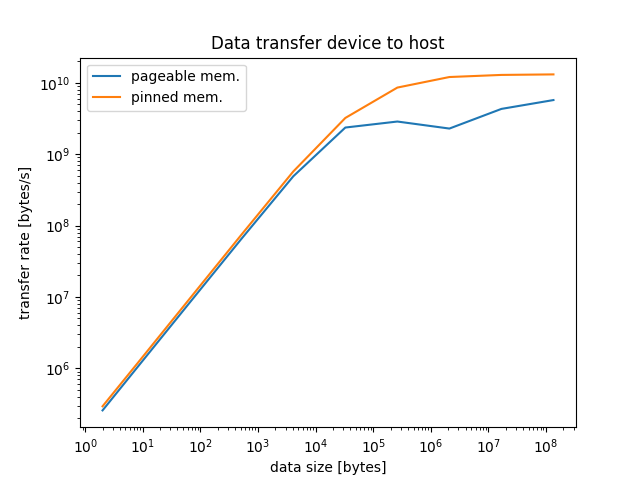
\includegraphics[scale=0.7]{data_d2h.png}
  \caption{Device to Host: pinned vs. pageable memory}
  \label{fig:203PCIe}
\end{figure}

\begin{figure}[h!]
  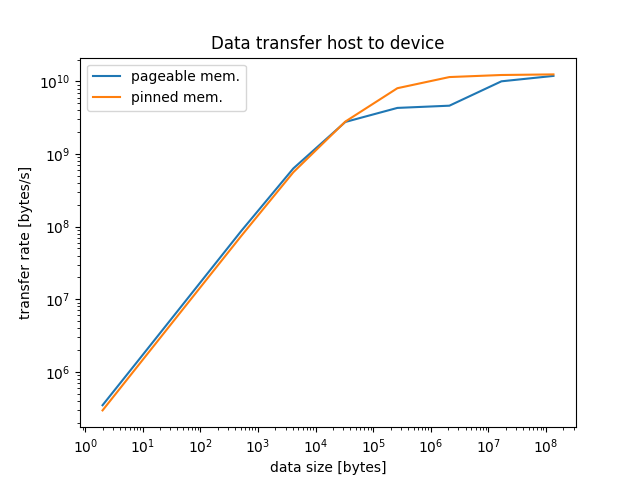
\includegraphics[scale=0.7]{data_h2d.png}
  \caption{Host to Device: pinned vs. pageable memory}
  \label{fig:204PCIe}
\end{figure}
